
\begin{frame}[fragile]
\frametitle{\lstinline{If}-Anweisung}
\begin{itemize}
\item Aus der Mathematik kennt man eine \glqq{}Zuweisung\grqq{} der
  folgenden Art.

Für $x\in\mathbb{R}$ setze
\begin{equation*}
y = |x| = \left\{\begin{array}{ll}
x & \text{falls $x\geq 0$}\\
-x & sonst
\end{array}\right.
\end{equation*}
\item Dies realisiert man in C++ mit einer \lstinline{If}-Anweisung:
{\scriptsize\begin{lstlisting}{}
double x(3.14), y;
if (x>=0)
{
  y = x;
}
else
{
  y = -x;
}
\end{lstlisting}}
\end{itemize}
\end{frame}

\begin{frame}[fragile]
\frametitle{Varianten der \lstinline{If}-Anweisung}
\begin{itemize}
\item Die geschweiften Klammern kann man weglassen, wenn der Block nur
  eine Anweisung enthält:
{\scriptsize\begin{lstlisting}{}
double x(3.14), y;
if (x>=0) y = x; else y = -x;
\end{lstlisting}}
\item Der \lstinline{else}-Teil ist optional:
{\scriptsize\begin{lstlisting}{}
double x=3.14;
if (x<0)
  std::cout << "x ist negativ!" << std::endl;
\end{lstlisting}}
\item Weitere Vergleichsoperatoren sind \lstinline{< <= == >= > !=}\\
\item Beachte: \lstinline{=} für Zuweisung, aber \lstinline{==} für den
Vergleich zweier Objekte!
\end{itemize}
\end{frame}


\subsection{Wiederholung}

\begin{frame}[fragile]
\frametitle{\lstinline{While}-Schleife}
\begin{itemize}
\item Bisher: Sequentielle Abfolge von Befehlen wie im Programm
  angegeben. Das ist langweilig :-)
\item Eine Möglichkeit zur Wiederholung bietet die
  \lstinline{While}-Schleife:

\lstinline{while (} \textsl{Bedingung} \lstinline{)}

\lstinline!{! \textsl{Schleifenkörper} \lstinline!}!

\item Beispiel:
{\scriptsize\begin{lstlisting}{}
int i=0; while (i<10) { i=i+1; }
\end{lstlisting}}

\item Bedeutung:
\begin{enumerate}
\item Teste Bedingung der \lstinline{While}-Schleife
\item Ist diese \textsl{wahr} dann führe Anweisungen im
  Schleifenkörper aus, sonst gehe zur ersten Anweisung nach dem
  Schleifenkörper.
\item Gehe nach 1.
\end{enumerate}
\item Anweisungen im Schleifenkörper beeinflussen normalerweise den Wahrheitswert der
  Bedingung.
\item Endlosschleife: Wert der Bedingung wird nie \textsl{falsch}.
\end{itemize}
\end{frame}


\begin{frame}[fragile]
\frametitle{Pendel (analytische Lösung; \lstinline{while}-Schleife)}
\begin{itemize}
\item Die Auslenkung des Pendels mit der Näherung
  $\sin(\phi)\approx\phi$ und $\phi(0)=\phi_0$, $\phi'(0)=0$ lautet:
$$ \phi(t) = \phi_0 \cos\left(\sqrt{\frac{g}{l}} t\right) .$$
\item Das folgende Programm gibt diese Lösung zu den Zeiten $t_i=i
  \Delta t$, $0\leq t_i \leq T$, $i\in\mathbb{N}_0$ aus:
\end{itemize}
\end{frame}
\begin{frame}[fragile]
\frametitle<presentation>{Pendel (analytische Lösung, \lstinline{while}-Schleife)}
\lstinputlisting[basicstyle=\ttfamily\scriptsize,numbers=left,
numberstyle=\tiny, numbersep=5pt]{../examples/progkurs/pendelwhile.cc}
\end{frame}

\begin{frame}[fragile]
\frametitle{Wiederholung (for-Schleife)}
\begin{itemize}
\item Möglichkeit der Wiederholung: \lstinline{for}-Schleife:

\lstinline{for (} \textsl{Anfang}; \textsl{Bedingung};
\textsl{Inkrement} \lstinline{)}

\lstinline!{! \textsl{Schleifenkörper} \lstinline!}!
\item Beispiel:
{\scriptsize\begin{lstlisting}{}
for (int i=0; i<=5; i=i+1)
{
  std::cout << "Wert von i ist " << i << std::endl;
}
\end{lstlisting}}
\item Enthält der Block nur eine Anweisung dann kann man die
  geschweiften Klammern weglassen.
\item Die \textsl{Schleifenvariable} ist so nur innerhalb des
  Schleifenkörpers sichtbar.
\item Die \lstinline{for}-Schleife kann auch mittels einer
  \textsl{while}-Schleife realisiert werden und umgekehrt.
\end{itemize}
\end{frame}

\begin{frame}[fragile]
\frametitle{Pendel (analytische Lösung, \lstinline{for}-Schleife)}
\lstinputlisting[basicstyle=\ttfamily\scriptsize,numbers=left,
numberstyle=\tiny, numbersep=5pt]{../examples/progkurs/pendel.cc}
\end{frame}

\begin{frame}
\frametitle{Visualisierung mit \lstinline{Gnuplot}}
\begin{itemize}
\item \lstinline{Gnuplot} erlaubt einfache Visualisierung von Funktionen
  $f:\mathbb{R}\to\mathbb{R}$ und
  $g:\mathbb{R}\times\mathbb{R}\to\mathbb{R}$.
\item Für  $f:\mathbb{R}\to\mathbb{R}$ genügt eine zeilenweise Ausgabe
  von Argument und Funktionswert.
\item Umlenken der Ausgabe eines Programmes in eine Datei:\\
\lstinline{$ ./pendel > pendel.dat}
\item Starte \lstinline{gnuplot}\\
\lstinline{gnuplot> plot "pendel.dat" with lines}
\end{itemize}
\mode<presentation>{
\begin{center}
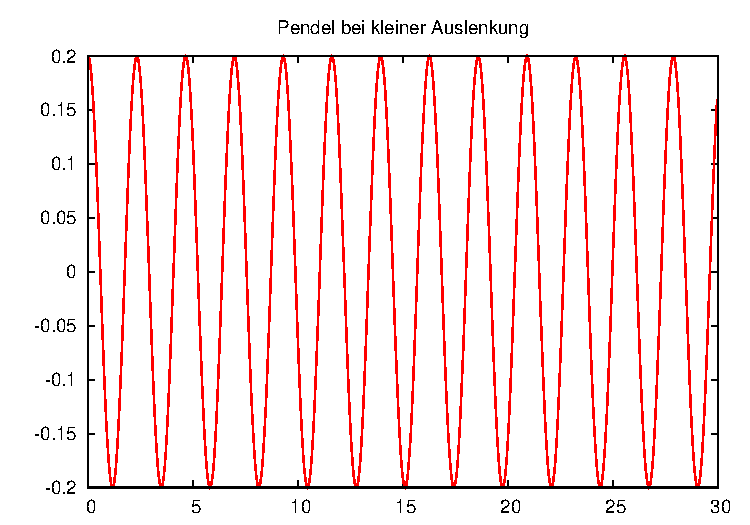
\includegraphics[width=0.4\textwidth]{./pendel}
\end{center}
}
\end{frame}

\note{Demonstration: Visualisierung mit Gnuplot.}

\begin{frame}[fragile]
\frametitle{Aufgabe 3}
\begin{enumerate}
\item Gebt eine Wertetabelle für  f(x) = $x^2$ im Bereich [-50 ,50] aus.
\item Orientiert euch dabei an pendel.cc für das Format der Ausgabe.
\item Plottet die Funktion mit Gnuplot. 
\end{enumerate}
\end{frame}
